\subsection{Computer}

Esta capa tiene como funcionalidades principales el manejo del ensamblado y la ejecución. 

\subsubsection*{Ensamblado}
El ensamblado permite, utilizando las rutinas que genera el translator, obtener el código binario de las instrucciones para luego poder ejecutarlo. 
En el proceso de ensamblado intervienen principalmente 4 clases: Computer, Instruction, State y Memory. En esta etapa, la clase Computer se encarga 
de recibir las rutinas a ensamblar y delega en las instrucciones de cada rutina la obtención del código binario para entregarlo a la clase State.
State se encarga de guardar en memoria el código binario de cada una de las instrucciones utilizando la clase Memory.

\begin{figure}[H]
  \centering
  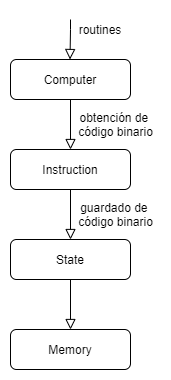
\includegraphics[width=3cm]{figuras/ensamblado.png}
  \caption{Proceso de ensamblado.}
\end{figure}

Como las instrucciones de una rutina pueden tener etiquetas o hacer uso de las mismas como operando, se definieron las clases Label y LabelReference 
para su manejo. Una rutina entonces, puede contener en su lista de instrucciones tanto elementos de tipo Instruction como de tipo Label.
El objetivo de la etapa de ensamblado es convertir las etiquetas en direcciones de memoria ya que las etiquetas son texto y este no puede ser
ensamblado en memoria. Para esto, el primer paso es calcular las direcciones de memoria donde se encuentren las definiciones de las etiquetas, es decir 
instancias de la clase Label. Luego, se deberán reemplazar los usos de esas etiquetas por operandos de tipo inmediato.

Para calcular las direcciones de memoria de las etiquetas se ven involucradas las clases Instruction y Label ya que son los elementos que puede
tener una rutina y el PC, que permite conocer la dirección de memoria actual. La clase Instruction, al solo representar instrucciones y no etiquetas, tiene la responsabilidad de avanzar el PC. Label en cambio,
tiene la responsabilidad de guardar el PC actual y su identificador en una lista de etiquetas y delegar en su instrucción el avance del PC.

\begin{figure}[H]
  \centering
  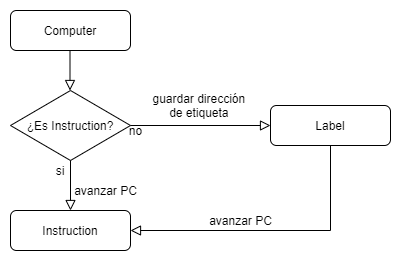
\includegraphics[width=8cm]{figuras/calculo-de-etiquetas.png}
  \caption{Cálculo de etiquetas.}
\end{figure}


\subsubsection*{Ejecución}

La etapa de ejecución se encarga de decodificar el código previamente ensamblado, traducirlo a instrucciones Q y ejecutarlas en orden.
De esta manera se da la noción de ejecución de un programa o rutina. Las instrucciones son decodificadas y ejecutadas de a una a la vez y esto permite
que el programa o rutina pueda mutar a lo largo de su ejecución. 

\begin{figure}[H]
  \centering
  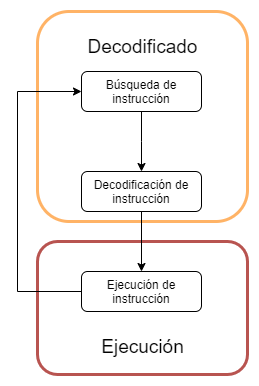
\includegraphics[width=4cm]{figuras/diagrama_ejecucion.png}
  \caption{Diagrama de ejecución.}
\end{figure}

Para ello, Computer lee la dirección de memoria indicada por el PC, cuyo contenido será decodificado. 
El decodificado del código máquina queda delegado en Instruction, ya que cada instrucción puede determinar si un código binario le corresponde y sabe
cómo decodificar sus operandos.
\begin{figure}[H]
  \centering
  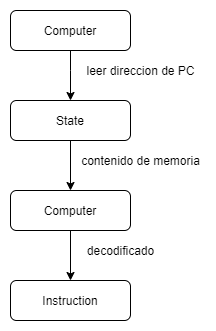
\includegraphics[width=5cm]{figuras/decodificado.png}
  \caption{Proceso de decodificado.}
\end{figure}

Una vez que la instrucción fue decodificada junto con sus operandos, se procede a ejecutarla. La ejecución de una instrucción recibe el estado actual y
lo modifica acorde a su efecto. Cada instrucción fue modelada con una clase, la cual conoce su efecto y lo aplica al ejecutarse. Este enfoque nos permite
agregar nuevas instrucciones facilmente siguiendo la interfaz brindada.

Estas modificaciones pueden incluir cambios en los flags, en el operando destino, en el PC o en la pila según la instrucción que se esté ejecutando.

Durante esta estapa pueden darse lecturas o escrituras de los operandos de origen y/o destino. Estos operandos pueden estar en modo inmediato, registro, directo,
indirecto o registro indirecto. Para conocer o modificar sus valores, los operandos dependen de los valores almacenados en el estado, quien guarda 
los valores de registros y conoce a la memoria. Es por ello que se definieron 5 clases para representar cada una de estas posibilidades, las cuales conocen
la forma de obtener valores del estado y guardarlos en él.

Como algunas instrucciones modifican los flags mientras que otras no lo hacen, esta tarea es delegada a cada instrucción, la cual conoce qué flags modifica
y cómo lo hace.

\begin{figure}[H]
  \centering
  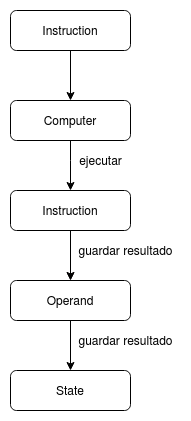
\includegraphics[width=4.5cm]{figuras/ejecucion_grafico.png}
  \caption{Proceso de ejecución.}
\end{figure}

\subsubsection*{La ejecución desde una mirada educativa}
En la definición de Q no existe la diferenciación de programa y rutina, como así tampoco la idea de finalización de ejecución. La computadora
está constantemente ejecucutando alguna instrucción, ya sea una instrucción con efecto o sin efecto.

Dado que QLib es una librería que simula una arquitectura de computadoras enfocada en la enseñanza, permite la creación de programas y rutinas. 
Estos se diferencian entre sí, porque los programas no finalizan con una instrucción RET mientras que las rutinas si. 

En la arquitectura Q no existe la idea de finalización de ejecución. Esto puede ser confuso para los/las estudiantes, ya que se esperaría que el programa tenga un inicio y 
un resultado final. Es por eso que consideramos que la librería debía proveer un método para identificar que la ejecución finalizó. 

Para ello, analizamos las siguientes condiciones: 

Al iniciar una ejecución las celdas que no hayan sido escritas, no tendrán valor. Por lo tanto el PC eventualmente llegará a una celda no incializada, esto puede darse por dos 
razones:
\begin{itemize}
  \item Un salto o una llamada a rutina en una celda vacía.
  \item Incremento orgánico del PC. Se considera que el PC se incrementó organicamente cuando su incremento no es causado por un offset o por una asignación directa.
\end{itemize}

Analizando dichas razones: 
\begin{itemize}
  \item Si se llega a una celda no inicializada mediante un salto o una llamada a rutina, asumimos que es un error de programación. Por ejemplo:
  \begin{center}
    MOV R1 R2 \\
    JMP 0x0fff \\
    \begin{footnotesize}
      En este caso se salta a la celda 0x0fff que no fue previamente inicializada.
    \end{footnotesize}
  \end{center}

  \begin{center}
    MOV R3 R0 \\
    CALL 0xAFFF \\
    \begin{footnotesize}
      En este caso se llama a la rutina ensamblada en la celda 0xAFFF que no fue previamente inicializada.
    \end{footnotesize}
  \end{center}

  \item Si se llega a una celda no inicializada mediante un incremento orgánico del PC pueden darse dos casos:
  
  La pila no está vacía, por lo tanto asumimos un error de programación. Posiblemente por el olvido de un RET.
  \begin{center}
    MOV R3 R0 \\
    CALL rutina \\
    MOV R0 R1 \\
  \end{center}
  \begin{center}
    [ASSEMBLE: 0x00ff] \\
    rutina: MOV R2 R3
  \end{center}
  
  La pila está vacía, puede haber dos razones:

  La etapa de ejecución no es \textit{FETCH} \footnote{FETCH es la etapa de la ejecución donde se busca en memoria la próxima instrucción a ejecutar.}. 
  \begin{center}
    MOV R3 [R0] \\
    \begin{footnotesize}
      En este caso, se lee el indirecto registro R0, pero la celda a la que apunta R0 no fue inicializada. Si bien esto no es un error, el resultado puede ser inesperado.
    \end{footnotesize}
  \end{center}
    
  La etapa de ejecución es FETCH, por lo tanto el programa finalizó.
  \begin{center}
    MOV R3 R0 \\
    CALL rutina \\
    MOV R0 R1 \\
  \end{center}
  \begin{center}
    [ASSEMBLE: 0x00ff] \\
    rutina: MOV R2 R3 \\
    RET
  \end{center}
\end{itemize}

\begin{samepage}
  Concluyendo, se asume la finalización de la ejecución cuando:
  \begin{itemize}
    \item La celda leída está no inicializada.
    \item El PC no fue modificado mediante un salto o una llamada a rutina.
    \item La pila se encuentra vacía.
    \item La etapa de ejecución es FETCH.
  \end{itemize}
\end{samepage}

\begin{figure}[H]
  \centering
  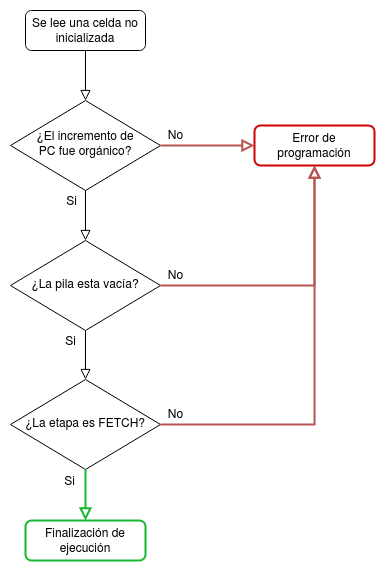
\includegraphics[width=7cm]{figuras/condicion_finalizacion.png}
  \caption{Condiciones de finalización.}
\end{figure}
\label{subsec:condfin}

Antes de definir una condición de finalización, tuvimos en cuenta la posibilidad de agregar una instrucción de fin, donde por ejemplo,
el usuario podría hacer uso de esta para definir cuándo o dónde el programa terminaría su ejecución.

Ejemplo de programa con instrucción de fin:
\begin{center}
  MOV R3 R0 \\
  ADD R0 R1 \\
  FIN \\
\end{center}

Con esta instrucción ya no sería necesario identificar una condición de finalización.

Optamos por definir una condición de finalización ya que esta facilita el entendimiento de un alumno o alumna de cuál es el resultado del 
programa que esté ejecutando abstrayendo la idea de que la computadora nunca deja de ejecutar. Por otro lado se evita agregar una instrucción que no 
se encuentra en Q.


\subsubsection*{QConfig}
\label{subsec:qconfig}
Existen distintos aspectos en QSim Web que pueden ser configurados con el objetivo de lograr que la herramienta tenga un enfoque más educativo y a su vez, 
para poder crear subconjuntos del lenguaje. QConfig es la clase encargada de guardar y modificar la configuración elegida. Existen las siguientes 
configuraciones:

\begin{itemize}
  \item Cantidad de registros: Permite modificar la cantidad de registros entre 1 y 8 (R0-R7). Si se intenta usar un registro deshabilitado, la 
  herramienta arrojará un error especificando lo sucedido.
  \item Comportamiento de la instrucción MUL: Permite elegir si se quiere que los 16 bits más significativos de una multiplicación se guarden en R7 o no.
  Esto es interesante ya que al principio resulta difícil de entender por los alumnos y que esté habilitado agregaría una complejidad esencial no 
  buscada en los comienzos de la materia.
  \item Valor por defecto en celdas: Permite elegir si el valor por defecto de una celda será cero; un error, si se intenta acceder al valor de una 
  celda no inicializada la herramienta lanzará una excepción; aleatorio, todas las celdas de memoria comenzarán con un valor aleatorio, 
  ayudando así a simular que la memoria siempre puede contener valores inesperados.
  \item Valor por defecto en registros: Permite elegir si el valor por defecto de un registro será cero o aleatorio.
  \item Modos de direccionamiento: Permite elegir qué modos de direccionamiento estarán habilitados en la ejecución. Si se intenta usar un modo de direccionamiento 
  deshabilitado, la herramienta lanzará una excepción indicando lo sucedido. 
  \item Instrucciones: Permite elegir qué instrucciones estarán habilitadas en la ejecución. Si se intenta usar una instrucción 
  deshabilitada, la herramienta lanzará una excepción indicando lo sucedido. 
\end{itemize}

Por ejemplo, si solo se requiere de Q1, basta con habilitar únicamente las instrucciones MOV, MUL, ADD, SUB y DIV y los modos de direccionamiento Inmediato y Registro.